\documentclass[12pt, letterpaper]{article}
\usepackage[T1,T2A]{fontenc}
\usepackage[russian]{babel}
\usepackage[utf8]{inputenc}
\usepackage{amsmath}
\DeclareMathOperator\erf{erf}
\usepackage{listings}
\usepackage{xcolor, graphicx}
\usepackage{tikz}

\title{Отчёт по лабораторной работе №22 по курсу “Языки и методы программирования”}
\author{Иван Кочкожаров}
\begin{document}
\maketitle
\noindent \textbf{Студент группы:} \underline{М80-108Б-22 Кочкожаров Иван Вячеславович, № по списку 25}    
\\
\textbf{Контакты e-mail:} \underline{tegusigaalpa@gmail.com}
\\
\textbf{Работа выполнена:} \underline{«31» марта 2023 г.}
\\
\textbf{Преподаватель:} \underline{асп. каф. 806 Сахарин Никита Александрович}
\\
\textbf{Входной контроль знаний с оценкой:} 5
\\
\textbf{Отчет сдан} \underline{«1» апреля 2023 г.}, \textbf{итоговая оценка:} 5
\\
\textbf{Подпись преподавателя:} \underline{\hspace{3cm}}
\section{Тема}
Издательская система \TeX{}.
\section{Цель работы}
Получить навыки оформления документов в издательской системе \LaTeX{}.
\section{Задание}
Оформить доклад об изучении \LaTeX{} на \LaTeX{}.
\section{Оборудование}
\noindent \textbf{Процессор:} AMD Ryzen 5 5600H (12) @ 3.300GHz
\\
\textbf{ОП:} 16gb
\\
\textbf{SSD:} 512 Gb SSD
\\
\textbf{Монитор:} 15.6" - 1920*1080
\\
\textbf{Графика:} Radeon RX Vega 7
\section{Программное обеспечение}
\noindent \textbf{Операционная система семейства:} Gentoo Linux x86-64
\\
\textbf{Интерпретатор команд:} bash версия 5.1.16
\\
\textbf{Текстовый редактор:} Visual Studio Code версия 1.76.0
\\
\textbf{Просмотрщик pdf:} zathura v. 0.5.1
\section{Идея, метод, алгоритм решения задачи}
Прочитать документацию \LaTeX{} и переписать отчет с Markdown на \LaTeX{}. tex-файл скомпилировать с помощью утилиты pdflatex.
\section{Сценарий выполнения работы}
Продемонстрируем широкий функционал \LaTeX{} на следующих примерах.
\subsection{Пример формул}
\[\cos (2\theta) = \cos^2 \theta - \sin^2 \theta\]
\[\lim\limits_{x \to \infty} \exp(-x) = 0\]
\[A=
\begin{pmatrix}
1 & 2 & 3\\
a & b & c
\end{pmatrix}\]
\[
\erf(x)=\frac{2}{\sqrt{\pi}}\int_{0}^{x}e^{-t^{2}}\, dt
\]
\subsection{Пример графиков gnuplot}
% GNUPLOT: LaTeX picture with Postscript
\begingroup
  \makeatletter
  \providecommand\color[2][]{%
    \GenericError{(gnuplot) \space\space\space\@spaces}{%
      Package color not loaded in conjunction with
      terminal option `colourtext'%
    }{See the gnuplot documentation for explanation.%
    }{Either use 'blacktext' in gnuplot or load the package
      color.sty in LaTeX.}%
    \renewcommand\color[2][]{}%
  }%
  \providecommand\includegraphics[2][]{%
    \GenericError{(gnuplot) \space\space\space\@spaces}{%
      Package graphicx or graphics not loaded%
    }{See the gnuplot documentation for explanation.%
    }{The gnuplot epslatex terminal needs graphicx.sty or graphics.sty.}%
    \renewcommand\includegraphics[2][]{}%
  }%
  \providecommand\rotatebox[2]{#2}%
  \@ifundefined{ifGPcolor}{%
    \newif\ifGPcolor
    \GPcolorfalse
  }{}%
  \@ifundefined{ifGPblacktext}{%
    \newif\ifGPblacktext
    \GPblacktexttrue
  }{}%
  % define a \g@addto@macro without @ in the name:
  \let\gplgaddtomacro\g@addto@macro
  % define empty templates for all commands taking text:
  \gdef\gplbacktext{}%
  \gdef\gplfronttext{}%
  \makeatother
  \ifGPblacktext
    % no textcolor at all
    \def\colorrgb#1{}%
    \def\colorgray#1{}%
  \else
    % gray or color?
    \ifGPcolor
      \def\colorrgb#1{\color[rgb]{#1}}%
      \def\colorgray#1{\color[gray]{#1}}%
      \expandafter\def\csname LTw\endcsname{\color{white}}%
      \expandafter\def\csname LTb\endcsname{\color{black}}%
      \expandafter\def\csname LTa\endcsname{\color{black}}%
      \expandafter\def\csname LT0\endcsname{\color[rgb]{1,0,0}}%
      \expandafter\def\csname LT1\endcsname{\color[rgb]{0,1,0}}%
      \expandafter\def\csname LT2\endcsname{\color[rgb]{0,0,1}}%
      \expandafter\def\csname LT3\endcsname{\color[rgb]{1,0,1}}%
      \expandafter\def\csname LT4\endcsname{\color[rgb]{0,1,1}}%
      \expandafter\def\csname LT5\endcsname{\color[rgb]{1,1,0}}%
      \expandafter\def\csname LT6\endcsname{\color[rgb]{0,0,0}}%
      \expandafter\def\csname LT7\endcsname{\color[rgb]{1,0.3,0}}%
      \expandafter\def\csname LT8\endcsname{\color[rgb]{0.5,0.5,0.5}}%
    \else
      % gray
      \def\colorrgb#1{\color{black}}%
      \def\colorgray#1{\color[gray]{#1}}%
      \expandafter\def\csname LTw\endcsname{\color{white}}%
      \expandafter\def\csname LTb\endcsname{\color{black}}%
      \expandafter\def\csname LTa\endcsname{\color{black}}%
      \expandafter\def\csname LT0\endcsname{\color{black}}%
      \expandafter\def\csname LT1\endcsname{\color{black}}%
      \expandafter\def\csname LT2\endcsname{\color{black}}%
      \expandafter\def\csname LT3\endcsname{\color{black}}%
      \expandafter\def\csname LT4\endcsname{\color{black}}%
      \expandafter\def\csname LT5\endcsname{\color{black}}%
      \expandafter\def\csname LT6\endcsname{\color{black}}%
      \expandafter\def\csname LT7\endcsname{\color{black}}%
      \expandafter\def\csname LT8\endcsname{\color{black}}%
    \fi
  \fi
    \setlength{\unitlength}{0.0500bp}%
    \ifx\gptboxheight\undefined%
      \newlength{\gptboxheight}%
      \newlength{\gptboxwidth}%
      \newsavebox{\gptboxtext}%
    \fi%
    \setlength{\fboxrule}{0.5pt}%
    \setlength{\fboxsep}{1pt}%
    \definecolor{tbcol}{rgb}{1,1,1}%
\begin{picture}(7200.00,5040.00)%
    \gplgaddtomacro\gplbacktext{%
      \csname LTb\endcsname%%
      \put(1285,1210){\makebox(0,0){\strut{}$-4$}}%
      \put(1932,1098){\makebox(0,0){\strut{}$-2$}}%
      \put(2579,985){\makebox(0,0){\strut{}$0$}}%
      \put(3226,873){\makebox(0,0){\strut{}$2$}}%
      \put(3872,761){\makebox(0,0){\strut{}$4$}}%
      \put(4618,833){\makebox(0,0)[l]{\strut{}$-4$}}%
      \put(4992,1027){\makebox(0,0)[l]{\strut{}$-2$}}%
      \put(5365,1222){\makebox(0,0)[l]{\strut{}$0$}}%
      \put(5739,1416){\makebox(0,0)[l]{\strut{}$2$}}%
      \put(6113,1611){\makebox(0,0)[l]{\strut{}$4$}}%
      \put(920,1990){\makebox(0,0)[r]{\strut{}$-1$}}%
      \put(920,2315){\makebox(0,0)[r]{\strut{}$-0.5$}}%
      \put(920,2638){\makebox(0,0)[r]{\strut{}$0$}}%
      \put(920,2963){\makebox(0,0)[r]{\strut{}$0.5$}}%
      \put(920,3288){\makebox(0,0)[r]{\strut{}$1$}}%
      \put(4195,3805){\makebox(0,0)[l]{\strut{}This is equal to 1}}%
    }%
    \gplgaddtomacro\gplfronttext{%
      \csname LTb\endcsname%%
      \put(5955,4316){\makebox(0,0)[r]{\strut{}$sinc(u,v)$}}%
      \csname LTb\endcsname%%
      \put(1864,408){\makebox(0,0){\strut{}X axis}}%
      \put(6318,704){\makebox(0,0){\strut{}Y axis}}%
      \put(-537,2638){\makebox(0,0){\strut{}Z axis}}%
      \csname LTb\endcsname%%
      \put(3600,4621){\makebox(0,0){\strut{}Sinc function}}%
    }%
    \gplbacktext
    \put(0,0){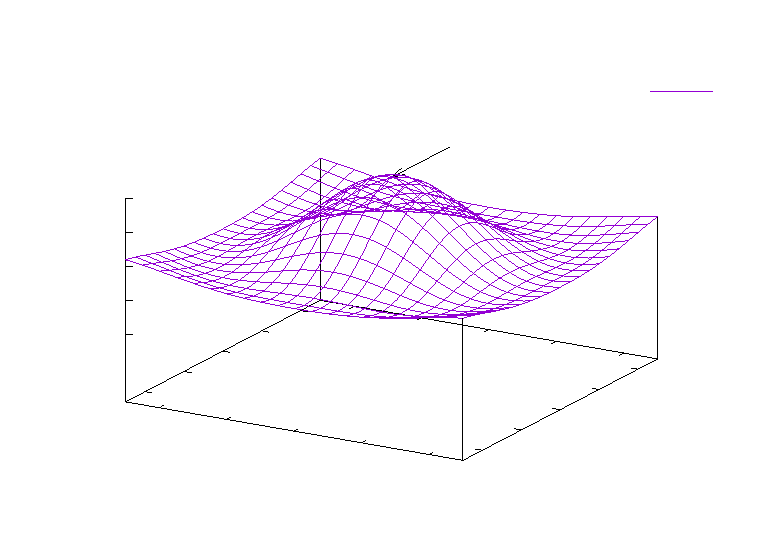
\includegraphics[width={360.00bp},height={252.00bp}]{plot}}%
    \gplfronttext
  \end{picture}%
\endgroup

\subsection{Пример графики}
\begin{figure}[h]
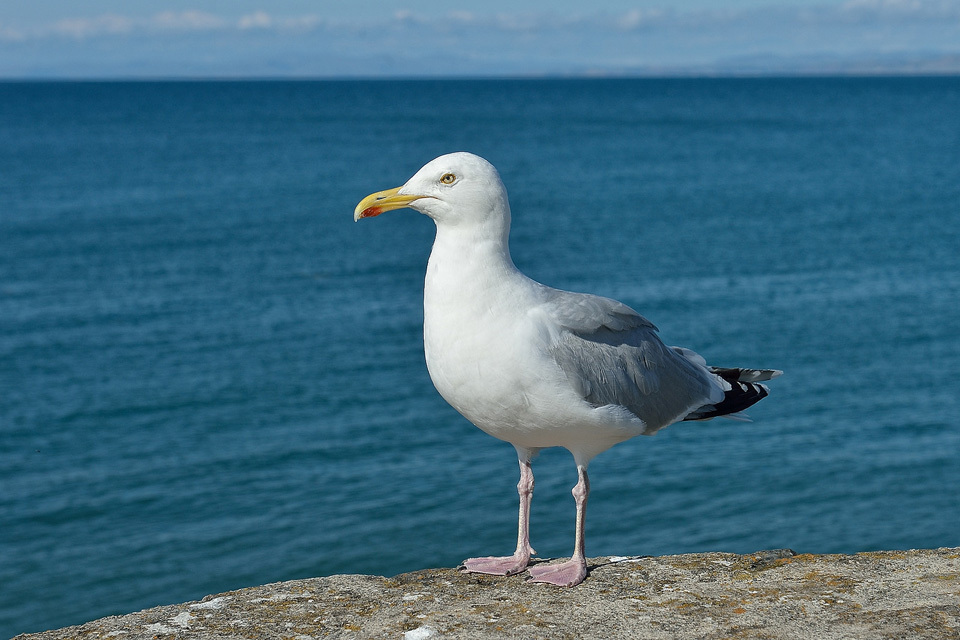
\includegraphics{gull}
\centering
\caption{Чайка}
\end{figure}
\begin{figure}[h]
\begin{tikzpicture}[>=stealth]
\draw[thick, ->, red] (0,0) -- (4,0);
\draw[thick, ->, red] (0,0) -- (1,3);
\draw[ultra thick, ->, blue] (0,0) -- (5,3);
\draw[dashed] (4,0) -- (5,3) -- (1,3);
\end{tikzpicture}
\centering
\caption{Сложение векторов}
\end{figure}
\section{Распечатка протокола}
\begin{lstlisting}[breaklines]
    This is pdfTeX, Version 3.141592653-2.6-1.40.22 (TeX Live 2021 Gentoo Linux) (preloaded format=pdflatex)
    restricted \write18 enabled.
    Output written on report.pdf (4 pages, 415766 bytes).
    Transcript written on report.log.
\end{lstlisting}  
\section{Дневник отладки}
\begin{tabular}{|c|p{1cm}|p{1.5cm}|c|p{2.5cm}|p{2cm}|p{2.25cm}|}
    \hline
    № & Лаб. или дом. & Дата & Время & Событие & Действие по исправлению & Примечание\\
    \hline
    1 & Дом. & 31.03.23-1.04.23 & 21:00 & Выполнение лабораторной работы & Свёрстан отчёт & -\\
    \hline
\end{tabular}
\section{Замечания автора по существу работы}
\section{Выводы}
\enlargethispage{-1\baselineskip}
Были получены навыки оформления докладов в издательской системе \LaTeX{}. Эта система продемонстрировала свою удобность для меня и в дальнейшем будет использована вместо MS Word для оформления курсовых работ по различным предметам. \\
\flushright \textbf{Подпись студента:} \underline{\hspace{3cm}}
\end{document}
